\subsection{Remote application configuration}\label{subsection:applied-methods:prototypical-implementation
:load-remote-settings}

The application shell is set up to use dynamic Module Federation. The location of the remote applications is determined at runtime. The problem with the so-called static Module Federation is that the \ac{URL} of the remote application must be known at build time. However, this is troublesome if the application should be built once and deployed to multiple stages. It is very cumbersome to build an artifact for every environment.

\bigskip

\noindent One possibility to fetch the remote definitions at runtime is to store them in a simple \ac{JSON} file, which can easily be configured for every environment. The host makes a simple GET request to get the definitions inside the \ac{JSON} file. The content of the file has to be a simple mapping between the name of the remote and their location, as shown in Listing \ref{code:applied-methods:define-module-federation-manifest}.

\ifshowListings
\begin{listing}[H]
\begin{minted}{json}
{
  "sales": "http://localhost:4201",
  "contact": "http://localhost:4202",
  "dashboard": "http://localhost:4203",
  "user": "http://localhost:4204"
}
\end{minted}
\caption{The structure of the micro-frontend definition file with the name and \ac{URL}.}\label{code:applied-methods:define-module-federation-manifest}
\end{listing}
\fi

\noindent The host has to fetch the definitions when starting up the application. The definitions are stored and stored for the Webpack configuration, as shown in Listing \ref{code:applied-methods:load-module-federation-settings}. If the file can be fetched successfully, the bootstrap process of the application gets imported dynamically.

\ifshowListings
\begin{listing}[H]
\begin{minted}{typescript}
fetch('/assets/module-federation.manifest.json')
  .then((res) => res.json())
  .then((definitions) => setRemoteDefinitions(definitions))
  .then(() => import('./bootstrap').catch((err) => console.error(err)));
\end{minted}
\caption{Loading the micro-frontend definition file during initialization.}\label{code:applied-methods:load-module-federation-settings}
\end{listing}
\fi

\noindent Another use case for dynamic content is the configuration of an application. This configuration includes the endpoint of the GraphQL \ac{API}, which can be different in staging and production. Therefore, the configuration should also be fetched dynamically. The settings are fetched during the first load of the application and stored for later use. The configuration is stored inside a file called \texttt{settings.json}, served alongside the application. Angular provides a handy mechanism to run code when the application is loaded.

\bigskip

\noindent With the help of the \texttt{APP\_INITIALIZER} injection token, asynchronous code can be executed when the application starts up. Such tasks include fetching data from a remote \ac{API} and setting up configuration or initializing third-party libraries. When an Angular app starts, it will execute all the functions registered with \texttt{APP\_INITIALIZER} in the order they were defined. If one of the initialization tasks fails, the application will not load. \cite{misc:-:applied-methods:prototype-implementation:angular-app-initializer}

\bigskip

\noindent The Listing \ref{code:applied-methods:fetch-and-store-settings} shows a simplified version to fetch and store the settings in the local storage. The settings are fetched from the \texttt{settings.json} file, which content is used to configure the application. The settings of the application shell are stored with the key \texttt{host}. Each application of the micro-frontend architecture stores its settings with its application name as the key.

\ifshowListings
\begin{listing}[H]
\begin{minted}{typescript}
@NgModule({
  providers: [{
    provide: APP_INITIALIZER,
    async useFactory(http: HttpClient, storage: StorageClient) {
      const environmentConfig = await lastValueFrom(
        http.get('assets/settings.json')
      );
      storage.store('host', environmentConfig);
    },
    multi: true,
    deps: [HttpClient, StorageClient],
  }]
})
class CoreModule {}
\end{minted}
\caption{Fetch \& store the settings of the application shell.}\label{code:applied-methods:fetch-and-store-settings}
\end{listing}
\fi

\subsubsection{Loading the configuration of the remote applications}\label{subsubsection:applied-methods:prototypical-implementation
:load-the-configuration}

Each application of the prototypical micro-frontend architecture follows this approach. When the application is initialized, the application configuration is fetched with a GET request from the \texttt{settings.json}. As mentioned in the previous section, each micro-frontend stores its settings with the application's name as the key. However, the configuration does not get fetched when the application shell consumes the functionality of a micro-frontend. Therefore, the application throws errors because they cannot access their settings from the storage. To solve the problem of missing settings for the application, the configuration of a remote application is fetched and stored inside a store when the user navigates to it. This procedure is explained visually in Figure \ref{fig:applied-methods:load-remote-settings}.

\ifshowImages
  \begin{figure}[H]
  \centering
  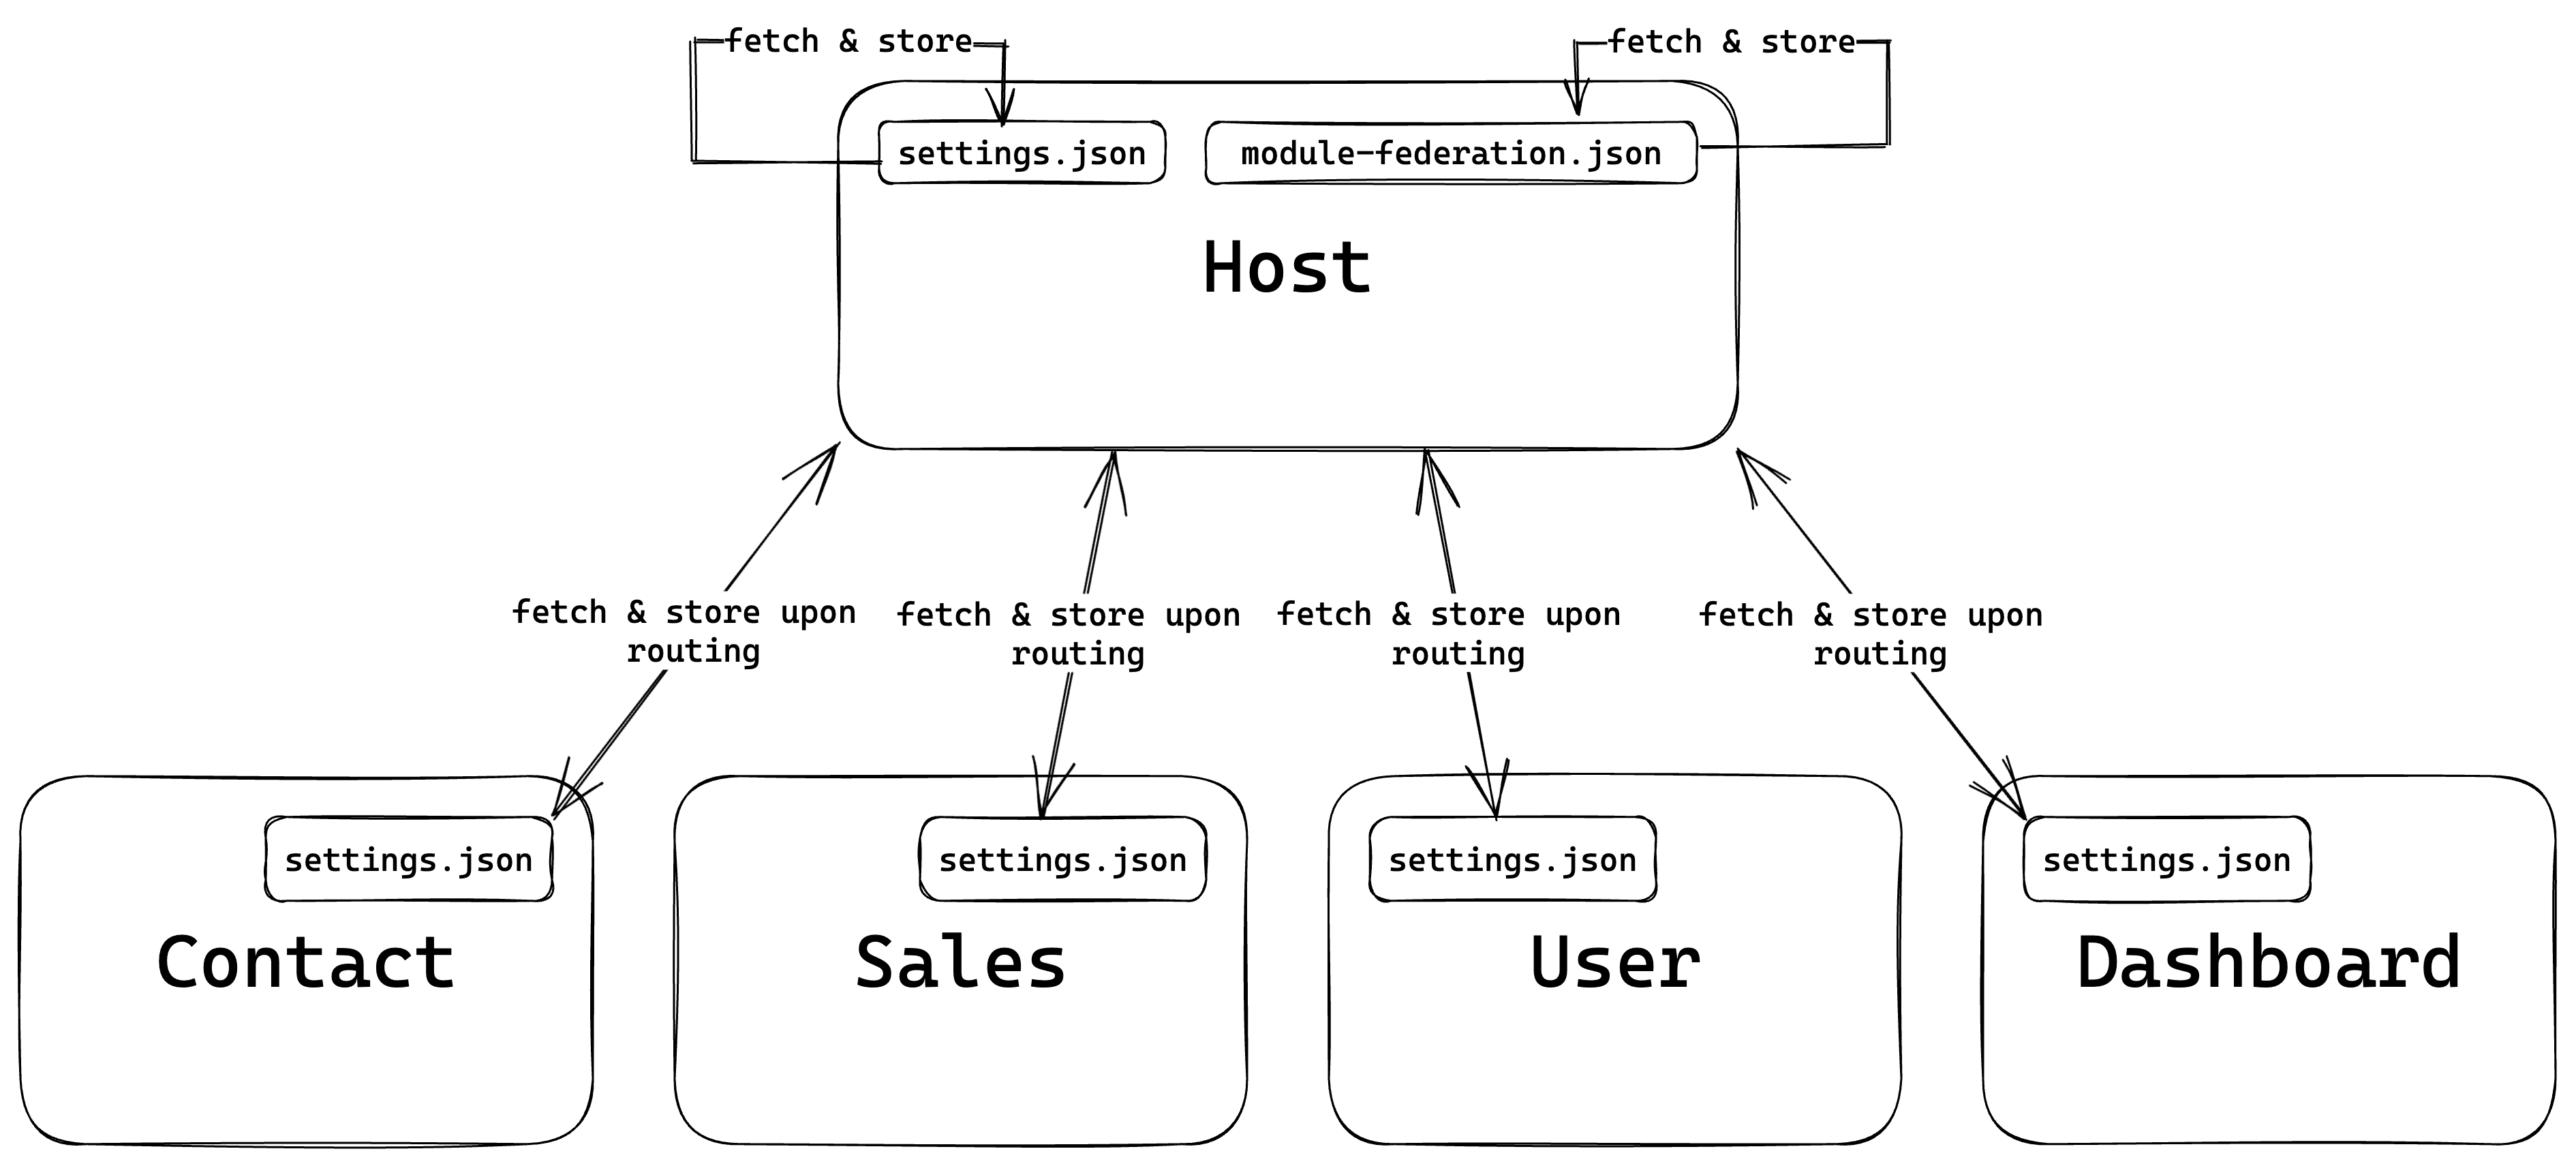
\includegraphics[width=0.9\linewidth]{images/applied-methods/prototypical-implementation/load-remote-settings.png}
  \caption{Loading a storing the configuration of the remote applications.}\label{fig:applied-methods:load-remote-settings}
  \end{figure}
\fi

\noindent With the help of Angular resolvers, the resolvers executed before the components of the target are rendered. Due to the dynamic Module Federation, the location of the remote module is known. Therefore, the \texttt{settings.json} is loaded and stored in addition to loading the remote module. A simplified version of the code is shown in Listing \ref{code:applied-methods:fetch-and-store-remote-application-settings}. The same principle applies to every remote module, which is consumed.

\ifshowListings
\begin{listing}[H]
\begin{minted}{typescript}
const routes: Routes = [{
    path: 'contact',
    loadChildren: () => loadRemoteModule('contact', './Module')
      .then((m) => m.ContactRemoteEntryModule),
    resolve: {
      settings: () => {
        const contact = inject(StorageClient).get('manifest')['contact'];
        return inject(HttpClient).get(`\${contact}/assets/settings.json`);
      }
    },
  },
  ...
]
\end{minted}
\caption{Fetch the settings of the contact application.}\label{code:applied-methods:fetch-and-store-remote-application-settings}
\end{listing}
\fi

\noindent With this approach, each application can access its settings like running in standalone mode. Moreover, it has another benefit because each application can only access its settings and not the settings of the other applications. 
